本アプリの依頼側、配達側、店舗側そして管理側の各機能設計について記述する。
\subsection{機能概要図}
以下に示す図は本アプリの機能概要である。

\subsubsection{ログイン関連機能}
図\ref{fig:ログイン関連機能}は、ログイン関連機能の概要図である。
\begin{figure}[H]
  \centering
  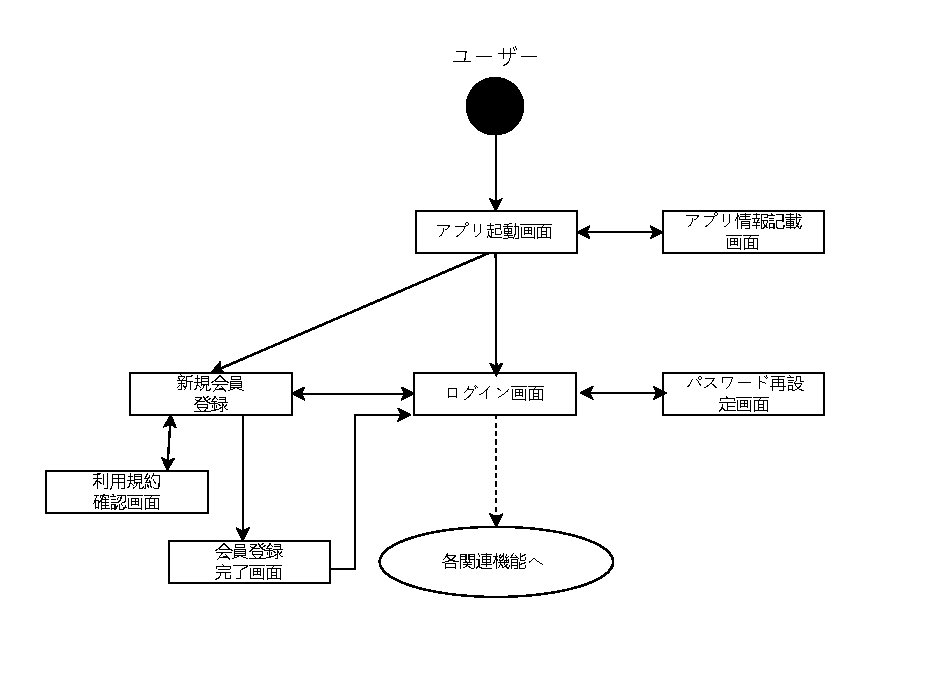
\includegraphics[width=0.75\textwidth]{./Image/ログイン関連機能.pdf}
  \caption{ログイン関連機能}
  \label{fig:ログイン関連機能}
\end{figure}



\subsection{共通機能}
本アプリの依頼側、配達側、店舗側そして管理側の共通の機能設計を以下に記述する。
\subsubsection{新規会員登録機能}
依頼側と配達側、店舗側が利用規約に同意し、情報を入力し、その情報に不備がなく、送信されたメールで本人確認を行うこ
とで、新規会員登録ができる機能である。また、入力情報として、配達側と依頼側は名前、性別、生年月日、住所、メールアドレス
、電話番号、パスワード、パスワード(確認)を、店舗側は店舗所在地、飲食店営業許可書のファイルおよび写真、メールア
ドレスまたは電話番号、パスワード、パスワード(確認)を入力する。

\begin{figure}[H]
  \centering
  \includegraphics[width=0.75\textwidth]{./Image/新規会員登録機能.pdf}
  \caption{新規会員登録機能}
  \label{fig:新規会員登録機能}
\end{figure}

\subsubsection{マイページ}
会員の情報を取得し、そのユーザが会員情報の確認・変更や、ログアウト、退会などが行える画面を表示させる機能で
ある。

\begin{figure}[H]
  \centering
  \includegraphics[width=0.75\textwidth]{./Image/マイページ機能.pdf}
  \caption{マイページ機能}
  \label{fig:マイページ機能}
\end{figure}

\subsubsection{ログイン}
アプリ起動時に会員登録済みの利用者(依頼側、配達側、店舗側そして管理側)が、自身のログイン情報を入力することで、
アプリのサービスを利用できるようにする機能である。依頼側、配達側、店舗側はメールアドレスとパスワードを、管理側は
管理者IDとパスワードを入力して、ログインする。

\begin{figure}[H]
  \centering
  \includegraphics[width=0.75\textwidth]{./Image/ログイン.pdf}
  \caption{ログイン機能}
  \label{fig:ログイン}
\end{figure}

\subsubsection{ログアウト}
ログアウトを選択することで、ログイン前の状態に戻す機能で、ログイン画面に遷移する。

\begin{figure}[H]
  \centering
  \includegraphics[width=0.75\textwidth]{./Image/ログアウト.pdf}
  \caption{ログアウト機能}
  \label{fig:ログアウト}
\end{figure}

\subsubsection{退会}
会員が任意のタイミングでアプリ会員から退会する機能。会員情報をデータベースから完全に削除する。

\begin{figure}[H]
  \centering
  \includegraphics[width=0.75\textwidth]{./Image/退会.pdf}
  \caption{退会機能}
  \label{fig:退会}
\end{figure}

\subsubsection{パスワード再発行}
ユーザーはパスワードを忘れた場合、メールアドレスをフォームに入力することで再発行を行う。間違っている場
合はエラーメッセージを出力し、合っている場合はパスワードを生成してデータベースを更新し、メールアドレス宛にそのパス
ワードを送信し、通知画面を表示する。

\begin{figure}[H]
  \centering
  \includegraphics[width=0.75\textwidth]{./Image/パスワード再発行.pdf}
  \caption{パスワード再発行機能}
  \label{fig:パスワード再発行}
\end{figure}

\subsubsection{会員情報確認・変更}
会員がアプリ内のホームページ画面から自身の会員情報を確認・変更するための機能である。

\begin{figure}[H]
  \centering
  \includegraphics[width=0.75\textwidth]{./Image/会員情報確認変更.pdf}
  \caption{会員情報確認・変更}
  \label{fig:会員情報確認変更}
\end{figure}

\subsubsection{問い合わせ}
会員がアプリの操作方法などの問い合わせを管理者に対して行うための機能である。
問い合わせへの回答は会員登録したメールアドレスに送信される。

\begin{figure}[H]
  \centering
  \includegraphics[width=0.75\textwidth]{./Image/問い合わせ機能.pdf}
  \caption{問い合わせ機能}
  \label{fig:問い合わせ機能}
\end{figure}

\subsection{依頼側}



\subsection{配達側}
\subsubsection{口座情報変更}
配達員が任意のタイミングで口座情報を変更する機能である。
\begin{figure}[H]
  \centering
  \includegraphics[width=0.75\textwidth]{./Image/deliverer機能設計/口座情報変更機能.pdf}
  \caption{口座情報変更機能}
  \label{fig:口座情報変更機能}
\end{figure}

\subsubsection{履歴書記述}
求人応募の際に必要となる履歴書情報を記述する機能である。
\begin{figure}[H]
  \centering
  \includegraphics[width=0.75\textwidth]{./Image/deliverer機能設計/履歴書記述機能.pdf}
  \caption{履歴書記述機能}
  \label{fig:履歴書記述機能}
\end{figure}

\subsubsection{マップ}
マップと配達ルートを表示する機能である。
\begin{figure}[H]
  \centering
  \includegraphics[width=0.75\textwidth]{./Image/deliverer機能設計/マップ.pdf}
  \caption{マップ機能}
  \label{fig:マップ}
\end{figure}

\subsubsection{求人検索}
求人検索する機能である。
\begin{figure}[H]
  \centering
  \includegraphics[width=0.75\textwidth]{./Image/deliverer機能設計/求人検索機能.pdf}
  \caption{求人検索機能}
  \label{fig:求人検索機能}
\end{figure}

\subsubsection{給与明細}
給与明細を表示する機能である。
\begin{figure}[H]
  \centering
  \includegraphics[width=0.75\textwidth]{./Image/deliverer機能設計/給与明細機能.pdf}
  \caption{給与明細表示機能}
  \label{fig:給与明細機能}
\end{figure}

\subsubsection{配達履歴}
配達履歴を表示する機能である。
\begin{figure}[H]
  \centering
  \includegraphics[width=0.75\textwidth]{./Image/deliverer機能設計/配達履歴.pdf}
  \caption{配達履歴表示機能}
  \label{fig:配達履歴}
\end{figure}

\subsubsection{配達員用通知}
配達用の通知を表示する機能である。
\begin{figure}[H]
  \centering
  \includegraphics[width=0.75\textwidth]{./Image/deliverer機能設計/deliverer通知機能.pdf}
  \caption{配達員用通知機能}
  \label{fig:deliverer通知機能}
\end{figure}


\subsection{店舗側}

\subsubsection{在庫ステータス変更機能}
商品の在庫の状況を変更する機能である。
\begin{figure}[H]
  \centering
  \includegraphics[width=0.75\textwidth]{./Image/administrator機能設計/アカウント情報登録機能.pdf}
  \caption{在庫ステータス変更機能}
  \label{fig:在庫ステータス変更機能}
\end{figure}

\subsubsection{メニュー登録機能}
店舗のメニューを登録する機能である。
\begin{figure}[H]
  \centering
  \includegraphics[width=0.75\textwidth]{./Image/administrator機能設計/アカウント情報登録機能.pdf}
  \caption{メニュー登録機能}
  \label{fig:メニュー登録機能}
\end{figure}

\subsubsection{メニュー削除機能}
メニューを削除する機能である。
\begin{figure}[H]
  \centering
  \includegraphics[width=0.75\textwidth]{./Image/administrator機能設計/アカウント情報登録機能.pdf}
  \caption{メニュー削除機能}
  \label{fig:メニュー削除機能}
\end{figure}

\subsubsection{メニュー情報変更機能}
メニュー情報を変更する機能である。
\begin{figure}[H]
  \centering
  \includegraphics[width=0.75\textwidth]{./Image/administrator機能設計/アカウント情報登録機能.pdf}
  \caption{メニュー情報変更機能}
  \label{fig:メニュー情報変更機能}
\end{figure}

\subsubsection{受注一覧}
受注一覧を表示する機能である。
\begin{figure}[H]
  \centering
  \includegraphics[width=0.75\textwidth]{./Image/administrator機能設計/アカウント情報登録機能.pdf}
  \caption{受注一覧機能}
  \label{fig:受注一覧機能}
\end{figure}

\subsubsection{配達員情報確認}
配達員の情報を確認する機能である。
\begin{figure}[H]
  \centering
  \includegraphics[width=0.75\textwidth]{./Image/administrator機能設計/アカウント情報登録機能.pdf}
  \caption{配達員情報確認機能}
  \label{fig:配達員情報確認機能}
\end{figure}

\subsubsection{受け渡し完了確認機能}
商品の受け渡し完了を確認する機能である。
\begin{figure}[H]
  \centering
  \includegraphics[width=0.75\textwidth]{./Image/administrator機能設計/アカウント情報登録機能.pdf}
  \caption{受け渡し完了確認機能}
  \label{fig:受け渡し完了確認機能}
\end{figure}

\subsubsection{配達トラブル報告機能}
配達に関するトラブルを報告する機能である。
\begin{figure}[H]
  \centering
  \includegraphics[width=0.75\textwidth]{./Image/administrator機能設計/アカウント情報登録機能.pdf}
  \caption{配達トラブル報告機能}
  \label{fig:配達トラブル報告機能}
\end{figure}


\subsubsection{売上確認機能}
売上に関する情報を確認する機能である。
\begin{figure}[H]
  \centering
  \includegraphics[width=0.75\textwidth]{./Image/administrator機能設計/アカウント情報登録機能.pdf}
  \caption{売上確認機能}
  \label{fig:売上確認機能}
\end{figure}


\subsubsection{売り上げ数確認機能}
売り上げ数に関する情報を確認する機能である。
\begin{figure}[H]
  \centering
  \includegraphics[width=0.75\textwidth]{./Image/administrator機能設計/アカウント情報登録機能.pdf}
  \caption{売り上げ数確認機能}
  \label{fig:売り上げ数確認機能}
\end{figure}


\subsubsection{明細表示機能}
売り上げや管理者への手数料を表示する機能である。
\begin{figure}[H]
  \centering
  \includegraphics[width=0.75\textwidth]{./Image/administrator機能設計/アカウント情報登録機能.pdf}
  \caption{明細表示機能}
  \label{fig:明細表示機能}
\end{figure}

\subsubsection{店舗用通知機能}
店舗用の通知を表示する機能である。
\begin{figure}[H]
  \centering
  \includegraphics[width=0.75\textwidth]{./Image/administrator機能設計/アカウント情報登録機能.pdf}
  \caption{店舗用通知機能}
  \label{fig:店舗用通知機能}
\end{figure}

\subsection{管理側}
\subsubsection{アカウント情報登録}
アカウント情報を登録する機能である。
\begin{figure}[H]
  \centering
  \includegraphics[width=0.75\textwidth]{./Image/administrator機能設計/アカウント情報登録機能.pdf}
  \caption{アカウント情報登録機能}
  \label{fig:アカウント情報登録機能}
\end{figure}
\subsubsection{アカウント情報削除}
アカウント情報を削除する機能である。
\begin{figure}[H]
  \centering
  \includegraphics[width=0.75\textwidth]{./Image/administrator機能設計/アカウント情報削除機能.pdf}
  \caption{アカウント情報削除機能}
  \label{fig:アカウント情報削除機能}
\end{figure}

\subsubsection{アカウント情報編集}
アカウント情報を編集する機能である。
\begin{figure}[H]
  \centering
  \includegraphics[width=0.75\textwidth]{./Image/administrator機能設計/アカウント情報編集機能.pdf}
  \caption{アカウント情報編集機能}
  \label{fig:アカウント情報編集機能}
\end{figure}

\subsubsection{アカウントID検索}
各種アカウント管理画面(依頼者、配達員、店舗、管理者)でアカウントIDを検索する機能である。
\begin{figure}[H]
  \centering
  \includegraphics[width=0.75\textwidth]{./Image/administrator機能設計/アカウントID検索機能.pdf}
  \caption{アカウントID検索機能}
  \label{fig:アカウントID検索機能}
\end{figure}

\subsubsection{アカウント名検索}
各種アカウント管理画面(依頼者、配達員、店舗、管理者)でアカウントの名前を検索する機能である。
\begin{figure}[H]
  \centering
  \includegraphics[width=0.75\textwidth]{./Image/administrator機能設計/アカウント氏名検索機能.pdf}
  \caption{アカウント名検索機能}
  \label{fig:アカウント名検索機能}
\end{figure}
\subsubsection{申請確認}
配達員や店舗から申請があったときに、申請の確認・承認を行う機能である。
\begin{figure}[H]
  \centering
  \includegraphics[width=0.75\textwidth]{./Image/administrator機能設計/申請確認機能.pdf}
  \caption{申請確認機能}
  \label{fig:申請確認機能}
\end{figure}
\subsubsection{依頼者アカウント管理画面表示}
依頼者アカウント管理画面の表示を行う機能である。
\begin{figure}[H]
  \centering
  \includegraphics[width=0.75\textwidth]{./Image/administrator機能設計/依頼者アカウント管理画面.pdf}
  \caption{依頼者アカウント管理画面表示機能}
  \label{fig:依頼者アカウント管理画面表示機能}
\end{figure}
\subsubsection{依頼者詳細表示}
依頼者アカウントの詳細の表示を行う機能である。
\begin{figure}[H]
  \centering
  \includegraphics[width=0.75\textwidth]{./Image/administrator機能設計/依頼者詳細表示機能.pdf}
  \caption{依頼者詳細表示機能}
  \label{fig:依頼者詳細表示機能}
\end{figure}
\subsubsection{配達員アカウント管理画面表示}
配達員アカウント管理画面の表示を行う機能である。
\begin{figure}[H]
  \centering
  \includegraphics[width=0.75\textwidth]{./Image/administrator機能設計/配達員アカウント管理画面.pdf}
  \caption{配達員アカウント管理画面表示機能}
  \label{fig:配達員アカウント管理画面表示機能}
\end{figure}
\subsubsection{配達員詳細表示}
配達員アカウントの詳細の表示を行う機能である。
\begin{figure}[H]
  \centering
  \includegraphics[width=0.75\textwidth]{./Image/administrator機能設計/配達員詳細表示機能.pdf}
  \caption{配達員詳細表示機能}
  \label{fig:配達員詳細表示機能}
\end{figure}

\subsubsection{履歴書表示}
配達員詳細画面から履歴書の表示を行う機能である。
\begin{figure}[H]
  \centering
  \includegraphics[width=0.75\textwidth]{./Image/administrator機能設計/履歴書表示.pdf}
  \caption{履歴書表示機能}
  \label{fig:履歴書表示}
\end{figure}
\subsubsection{警告通知}
配達員アカウントの詳細画面から警告通知を行う機能である。
\begin{figure}[H]
  \centering
  \includegraphics[width=0.75\textwidth]{./Image/administrator機能設計/警告通知機能.pdf}
  \caption{警告通知機能}
  \label{fig:警告通知機能}
\end{figure}





